\documentclass[class=NCU_thesis, crop=false]{standalone}

\begin{document}
\chapter{實驗架設與結果討論}
本章為實驗的主軸,會從光源的製備出發,說明實驗上會用到兩種不同光源的產生機制。再介紹光路的架設與其測量上限制,且會在同樣的架設下,分別以兩種不同的光源去測量,交叉驗證不同系統下實驗的結果,並與前幾章的理論計算比較,探討可能產生誤差的原因,以實際的狀況去修正理論模擬,讓計算結果更貼近測量數據,

\section{光源製備}

\subsection{雷射光}
雷射光源為 TOPTICA 的 DLC TA-SHG PRO 雷射系統,可產生中心波長約為 795 nm 的窄頻雷射。此雷射的特點為出光頻率可調,可以透過電壓控制共振腔上光柵的角度來調整出光的頻率。

除了波長 795 nm 的紅外,雷射系統內還有一塊在共振腔內的非線性晶體,可將前述的紅光打入內,產生倍頻效應 (SHG) 產生波長為 397.5 nm 的藍光,可用來打入另一塊非線性晶體,以自發參量下轉換 (Spontaneous Parametric Down-Conversion, SPDC) 的過程產生 975 nm 的光子。


\subsection{單光子}
\label{subsection:single_photon}
雙光子的產生機制為 SPDC,入射一道波長 397.5 nm 的藍光雷射進入 PPKTP 晶體,產生 Type-II 的時間 - 能量糾纏光子對 (time-energy entangled biphoton),波長為 795 nm。

藉由在 PPKTP 晶體雙邊鍍上 795nm 的高反射薄膜,右邊鍍上 397.5 nm 的高反射薄膜,可形成一個共振腔,讓產生出來的光子對有相對長的相干時間 (coherence time) 與較窄的頻寬。

實驗上會將產生出來的雙光子對經過 PBS,將訊號分為 signal 和 idler,以 idler 做為觸發訊號,使 signal 經過 $^{87}Rb$ 原子氣體管與 EOM,讓光子被吸收或對其進行相位的調製,並做 $G^{2}(\tau)$ 的測量,$G^{2}(\tau)$ 的定義如 (\ref{eq:g2_definition})。

\begin{equation}
    G^{2}(\tau)=\frac{4\Gamma_{s}\Gamma_{i}}{\Gamma_{s}+\Gamma_{i}}\left\{\begin{matrix}
        e^{\Gamma_{s}\tau} & ,\tau<0\\
        e^{-\Gamma_{i}\tau} & ,\tau>0
        \end{matrix}\right.
\label{eq:g2_definition}
\end{equation}

此為二階強度關聯函數 (second-order intenstiy correlation function),$\tau$ 為兩顆單光子抵達探測器的時間差。在符合準相位匹配條件 (quasi phase matching condition) 時能最有效率的產生雙光子,實際測量結果如\cref{fig:single_photon_g2},此光子之時間波包寬度約為 100 ns,頻寬為 4.5 MHz。

\fig[0.75][fig:single_photon_g2][!htb]{nocell_spread_no_etalon.png}[糾纏光子對之 $G^{2}(\tau)$ 量測]


為了找到符合準項未匹配條件的入射光波長與晶體溫度,實驗上我們先將入射光的頻率固定在 105489 MHz,改變晶體溫度測量雙光子的產生率 (biphton rate),結果如\cref{fig:temp_scan_g2}黑線,在 39.91$^{\circ}C$ 至 40.10$^{\circ}C$ 有四組符合條件的模態,若讓其中一顆光子經過 $^{87}Rb$ 原子氣體管,並做相同的量測,結果如\cref{fig:temp_scan_g2}紅線,可以發現第二和第三個的模態雖有明顯的吸收,但吸收率不高,我們認為這是因為晶體所產生的光子為多模 (multi-mode) 而非單模 (single-mode),同時產生了兩種以上頻率的單光子,儘管其中一個頻率的光子能完全被吸收,其他頻率的光子仍會透射,因此無法讓透射率趨近於零。為了確認這想法,我們在探測器前面加上一個頻寬為 60 MHz 的 Etalon 濾波器,只允許特定頻率附近的光通過,並在沒放 $^{87}Rb$ 原子氣體管時改變晶體溫度,重新測量產生率,有無 Etalon 濾波器測量之結果比較如\cref{fig:temp_scan_g2_with_etalon},黑色為沒放 Etalon 濾波器時測量到的訊號,紅色經過濾波後之訊號,兩者相比可明顯看出,有放濾波器時能將其他產生效率較低的模態過濾掉,一次只讓一個特定頻率區間內的光通過。此時再將 $^{87}Rb$ 原子氣體管放回,並對其中第二和第三個模態進行相同的量測,結果如\cref{fig:absorption_etalon_temp_scanning},黑線為加上 Etalon 過濾之後測到的訊號,若放上 $^{87}Rb$ 原子氣體管讓光子通過,測量結果如藍線,光子幾乎完全被吸收,與\cref{fig:temp_scan_g2}相比,可明顯看出,在過濾前的光源的確有其他頻率的成分,要避免其他頻率成分影響後續的實驗與分析,需加上 Etalon 濾波器。

\fig[0.75][fig:temp_scan_g2][!htb]{temp_scanning.png}[調整溫度測量雙光子產生率,黑線為直接對雙光子進行量測;紅線為先讓其中一顆單光子通過 $^{87}Rb$ 氣體管再測量,其中第二和第三個模態有部分吸收。][調整溫度測量雙光子產生率]

\fig[0.75][fig:temp_scan_g2_with_etalon][!htb]{temp_scanning_with_etalon.png}[黑色為無濾波器時測量之訊號,在二與三個模態附近測量到一些明顯的訊號,表示我們的單光子非單模;紅線為經過濾波器測量到的訊號,此時就只允許特定頻率透射。][調整溫度測量雙光子產生率(加上濾波器)]

\begin{figure}[!hbt]
    %\captionsetup[subfigure]{labelformat=empty} % 完全隱藏圖號
    \centering
    \subcaptionbox
        {第二個模態
        \label{fig:subfig_fig1}}
        {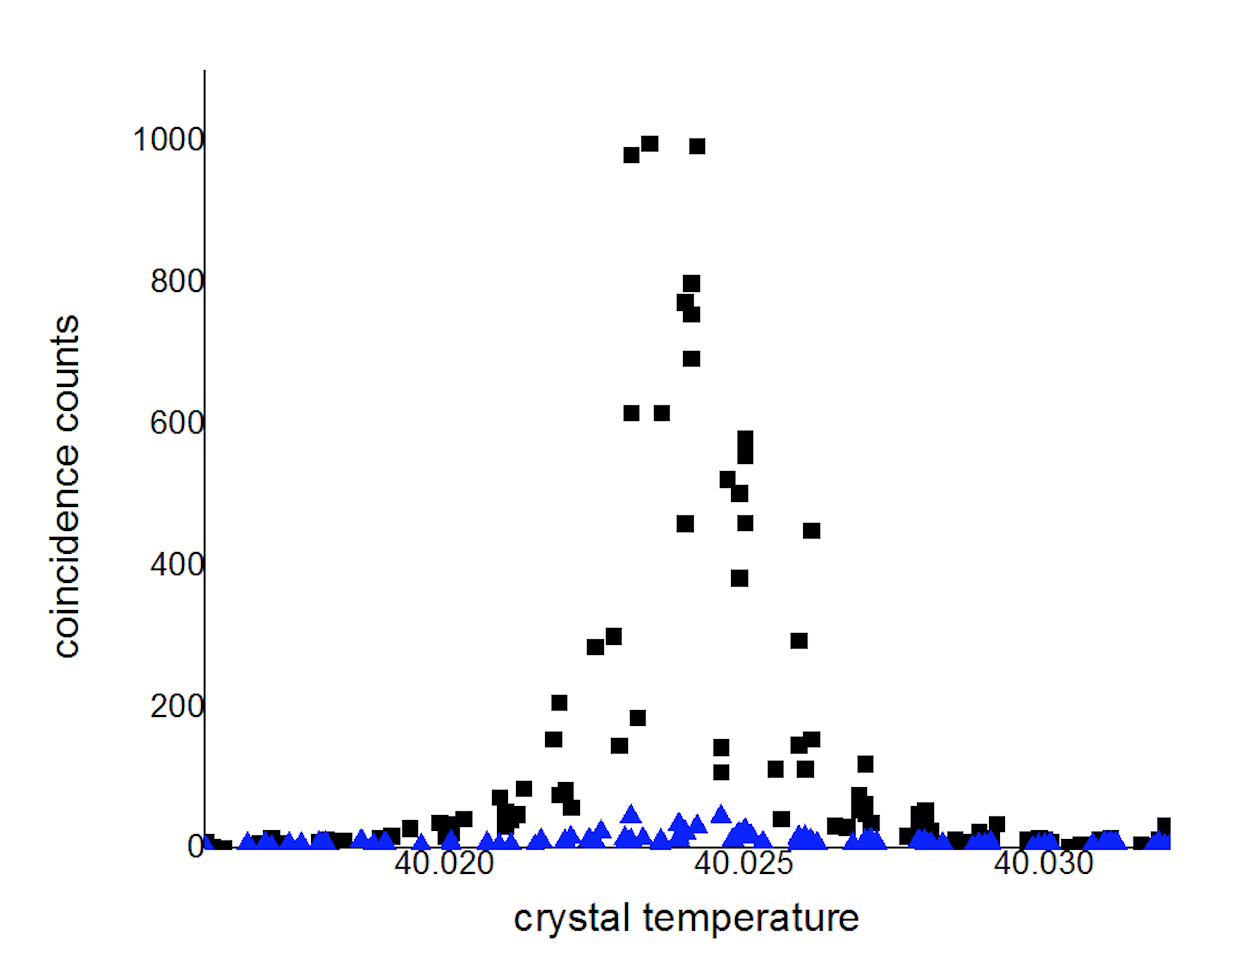
\includegraphics[width=0.4\linewidth]{second_mode_absorption.png}}
    ~~~~
    \subcaptionbox
        {第三個模態
        \label{fig:subfig_fig2}}
        {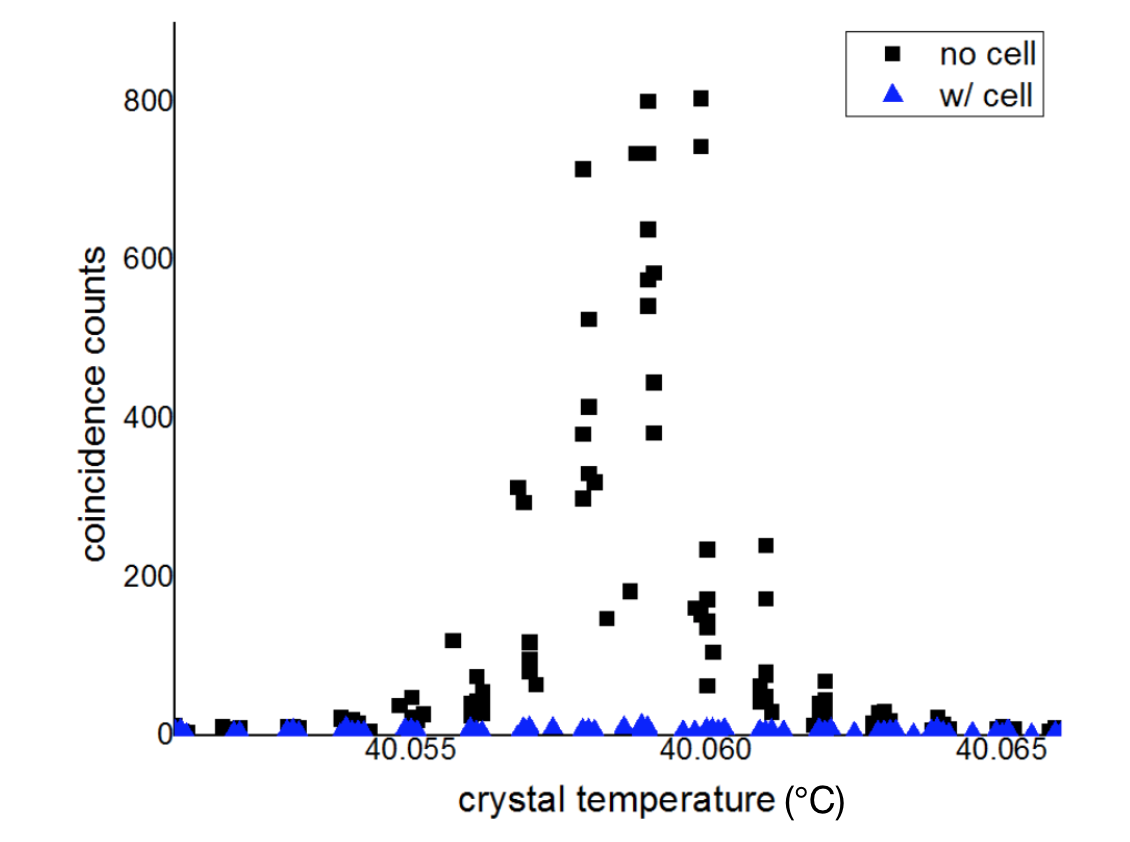
\includegraphics[width=0.4\linewidth]{third_mode_absorption.png}}
    \caption{經過 Etalon 濾波後光子之吸收}
    \label{fig:absorption_etalon_temp_scanning}
\end{figure}

\section{雷射頻譜量測}

實驗光路架設如\cref{fig:laser_spectrum_setup},我們將窄頻雷射通過兩台 EOM 對其進行相位調製,第一台為展頻用,第二台用來做反向的調製還原頻譜,再以 Fabrty-Perot 干涉儀去測量頻譜。

\fig[0.75][fig:laser_spectrum_setup][!htb]{laser_spectrum_setup.png}[雷射頻譜量測光路圖]

在兩台 EOM 都關閉的情況下,可以測到波長 795 nm 雷射的頻譜,結果如\cref{fig:laser_spectrum},以此 Fabry-Perot 的解析度掃出的雷射頻寬約為 60 MHz。

\fig[0.75][fig:laser_spectrum][!htb]{laser_spectrum.png}[以頻寬 60MHz 的 Fabry-Perot 干涉儀掃出之雷射頻譜][雷射頻譜]


若只開啟第一台 EOM,在 10 Gb/s 隨機訊號的調製下可將窄頻雷射光的頻譜展至 10 GHz 寬,但由於我們的使用的 Fabry-Perot FSR 僅 10 GHz,無法涵蓋完整的頻率區間,會使測量的結果失真,要想掃出完整展開的頻譜需使用 FSR 20 GHz 以上的干涉儀,所以下面會先以 2 Gb/s 的訊號來測試展頻的結果是否符合理論模擬。

\subsection{2 Gb/s 隨機訊號之相位調製}
先以 2 Gb/s 隨機訊號進行相位調製,只開啟第一台能將頻譜展至 $\pm$5 GHz 寬,如\cref{fig:2gbs_spread}。

\fig[0.75][fig:2gbs_spread][!htb]{2_31_spread_2GHz.png}[2 Gb/s 訊號之展頻頻譜]

頻譜的形狀大致上與理論相符,但在 $\pm$2 GHz 的位置有一個突起的訊號,這是由於隨機訊號的上升與下降時間不夠快所致,若在數值模擬中把隨機訊號加上約 35 ps 的上升與下降時間(如\cref{fig:simulation_rising_falling_prbs}),則會出現類似的結果,如\cref{fig:simulation_rising_falling}。

\begin{figure}[!hbt]
    %\captionsetup[subfigure]{labelformat=empty} % 完全隱藏圖號
    \centering
    \subcaptionbox
        {修正前之隨機訊號
        \label{fig:subfig_fig1}}
        {
\includegraphics[width=0.4\linewidth]{temp.png}}
    ~~~~
    \subcaptionbox
        {修正後展頻頻譜
        \label{fig:subfig_fig2}}
        {
\includegraphics[width=0.4\linewidth]{temp.png}}
    \caption{隨機訊號之上升與下降時間對頻譜之影響}
    \label{fig:simulation_rising_falling_prbs}
\end{figure}

\begin{figure}[!hbt]
    %\captionsetup[subfigure]{labelformat=empty} % 完全隱藏圖號
    \centering
    \subcaptionbox
        {上升與下降時間為 0 ps 之展頻模擬
        \label{fig:subfig_fig1}}
        {
\includegraphics[width=0.4\linewidth]{temp.png}}
    ~~~~
    \subcaptionbox
        {上升與下降時間為 35 ps 之展頻模擬
        \label{fig:subfig_fig2}}
        {
\includegraphics[width=0.4\linewidth]{temp.png}}
    \caption{隨機訊號之上升與下降時間對頻譜之影響,隨機訊號加了上升與下降時間後的模擬更貼近實驗結果。}
    \label{fig:simulation_rising_falling}
\end{figure}

\todo[inline]{隨機訊號模擬圖,展頻模擬圖}

此外,還可隱約看出該頻譜的包絡線有週期振盪的訊號,原因為我們使用的隨機訊號實際上是個重複出現的週期訊號,每個週期有 $2^{31}-1$ 個位元,若把位元數調為 $2^{15}-1$ 或者 $2^{7}-1$ 則可看到週期更大的震盪訊號,測量結果如\cref{fig:different_length_PRBS}。

\begin{figure}[!hbt]
    %\captionsetup[subfigure]{labelformat=empty} % 完全隱藏圖號
    \centering
    \subcaptionbox
        {週期 $2^{15}-1$ 位元之偽隨機訊號
        \label{fig:subfig_fig1}}
        {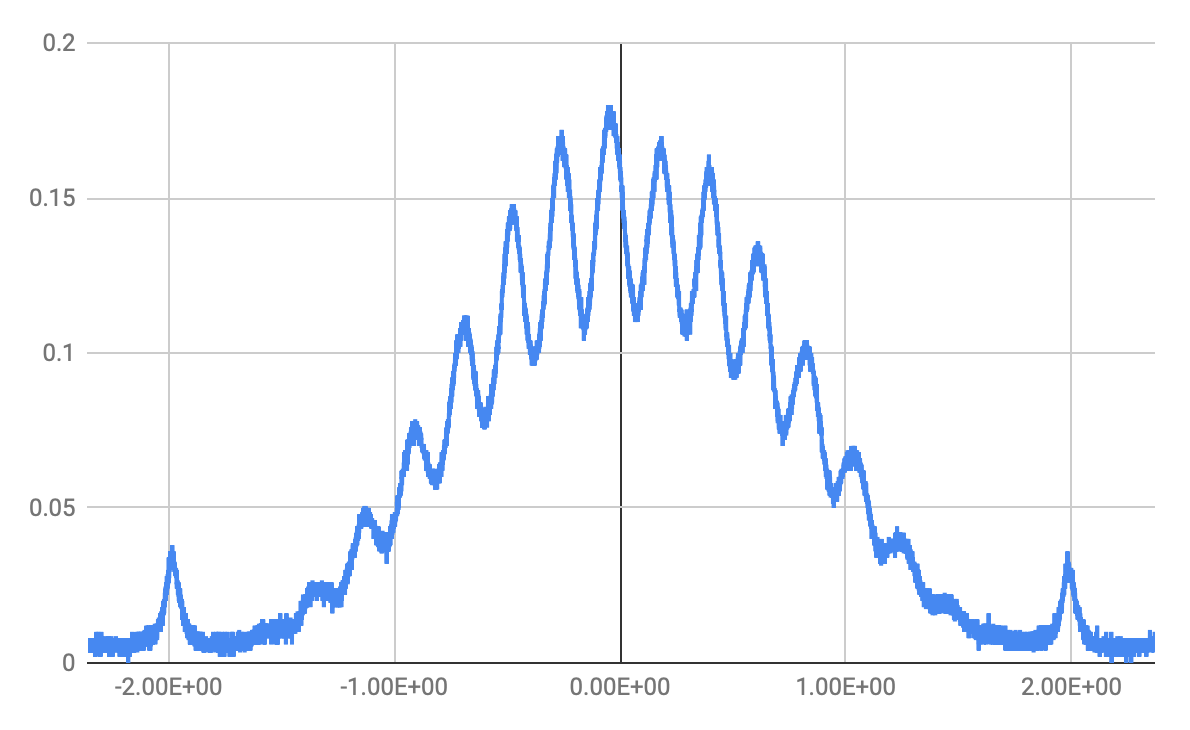
\includegraphics[width=0.4\linewidth]{2_7_spread_2GHz.png}}
    ~~~~
    \subcaptionbox
        {週期 $2^{7}-1$ 位元之偽隨機訊號
        \label{fig:subfig_fig2}}
        {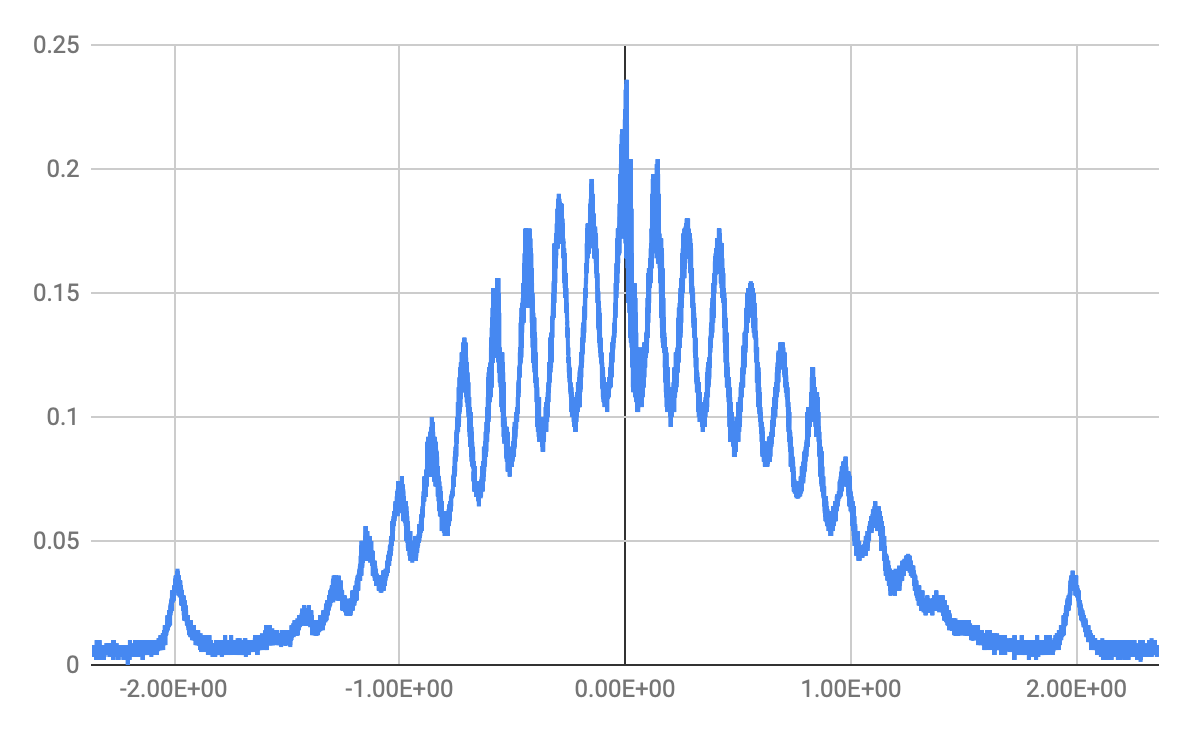
\includegraphics[width=0.4\linewidth]{2_15_spread_2GHz.png}}
    \caption{偽隨機訊號週期與展頻頻譜震盪之關係}
    \label{fig:different_length_PRBS}
\end{figure}

從以上測量的頻譜可以看出,調製後的頻寬與理論計算的結果一致,所以我們認為 10 Gb/s 的隨機訊號能將訊號展至 $\pm$10 GHz 寬。

\subsection{10 Gb/s 隨機訊號之相位調製}

當兩台 EOM 同時開啟時,理論上要能將展寬的頻譜還原成調製前的狀態,但從\cref{fig:10gbs_compress_sprectrum} 的實驗結果可以看出,壓縮回來的頻譜與調製前相比,中心頻率的強度僅為本來的 80\%,若將電壓放大來看(如\cref{fig:compress_amplified_compare})可以觀察到,在調製前所有能量皆集中於中心頻率附近,但經過兩台 EOM 調製後,仍有部分能量分散在其他頻率沒被還原,導致中心頻率的強度降低。造成頻譜還原效果不佳的可能原因為,兩個隨機訊號的形狀與穩定度皆不同(如\cref{fig:amplified_signal}),使相位無法被反向調製,還原成最初的狀態。

\fig[0.75][fig:10gbs_compress_sprectrum][!htb]{compress_comparison_100.png}[10 Gb/s 訊號壓縮後頻譜]

\fig[0.75][fig:compress_amplified_compare][!htb]{compress_zoom_in.png}[放大後之電訊號,紅線為未經調製的雷射頻譜,黑線為兩次調製後的訊號,雖能大致上將頻寬從 10 GHz 壓回 60 MHz,但從圖中可發現,中心以外的頻率仍能測到一些訊號。][初始頻譜與壓縮頻譜放大比較圖]

\begin{figure}[!hbt]
    %\captionsetup[subfigure]{labelformat=empty} % 完全隱藏圖號
    \centering
    \subcaptionbox
        {第一台 EOM 
        \label{fig:subfig_fig1}}
        {\includegraphics[width=0.4\linewidth]{amp_data.bmp}}
    ~~~~
    \subcaptionbox
        {第二台 EOM
        \label{fig:subfig_fig2}}
        {\includegraphics[width=0.4\linewidth]{amp_data_bar.bmp}}
    \caption{經過放大器,進入 EOM 用以調製的兩組隨機訊號眼圖}
    \label{fig:amplified_signal}
\end{figure}

\section{經相位調製後之 $^{87}Rb$ 原子吸收譜}

如\cref{section:simulation_absorption} 所提,當光子的頻率很接近原子的躍遷能階時,光會被吸收,實驗上可以\cref{fig:laser_spectrum_setup}的架設,將 Farby-Perot 干涉儀換成光二極體 (photodiode) 收光,連續調變入射光的頻率,測量透射 $^{87}Rb$ 原子氣體管的光強,從\cref{fig:abs_spec} 藍線可以觀察到,在特定的兩個頻率位置附近光會被原子吸收,穿透率特別低。本實驗主要的目的為透過展頻技術,降低光子與原子的交互作用,使光子能不被吸收而增加透射率,所以若將第一台 EOM 開啟,將雷射的頻寬從 60 MHz 展至 10 GHz,此時的吸收譜如\cref{fig:abs_spec} 紅線,在經過展頻後,無論在哪個頻率下光皆能大部分透射原子,調製前的光在 105 GHz 與 112 GHz 會被完全吸收,調製後卻有 75\% 的光能透射原子,就如隱形了一般,展頻能降低光子受環境的影響。

\fig[0.75][fig:abs_spec][!htb]{absorption_spectrum_spread.png}[調製後的如原子吸收譜,黑線為沒放 $^{87}Rb$ 原子氣體管時的訊號;藍線為調製前 $^{87}Rb$ 原子氣體管的吸收譜;紅線為展頻後的吸收譜。][調製後的銣原子吸收譜]

\section{單光子相位調製對原子吸收之影響}
從前一小節的實驗結果能得知,$^{87}Rb$ 的躍遷頻率約在 105 GHz 與 112 GHz 附近,這時我們將光源從窄頻雷射換成單光子,並透過改變入射光的頻率與晶體溫度,將單光子的頻率調至 112300 MHz,使其能被原子吸收,再以\cref{fig:single_photon_no_etalon} 的光路架設對光子進行相位調製與測量。

\fig[0.75][fig:single_photon_no_etalon][!htb]{single_photon_no_etalon_setup.png}[單光子量測光路圖]

當兩台 EOM 皆關閉時,頻寬約為 4.5 MHz 的單光子會幾乎完全被原子吸收,光無法透射氣體管,但若對其進行 $G^{2}(\tau)$ 測量,卻會測到訊號,如\cref{fig:remaining_mod_g2},原因如\cref{subsection:single_photon} 所述,是由於我們晶體產生的單光子源非單模 (single-mode),其中還存在符合其他組準相位匹配條件 (quasi phase matching condition) 所產生的光,若要去除那些光子對實驗的影響,在此小節的數據處理上,我們直接將其當作雜訊扣除,只保留主要模態的光;下一小節的實驗中,我們會外加一個 Etalon 濾波器,只讓 112300 MHz 附近的光通過。

\fig[0.75][fig:remaining_mod_g2][!htb]{initial_heatcell_no_etalon.png}[單光子通過 $^{87}Rb$ 原子氣體管之 $G^{2}(\tau)$ 量測,黑線為沒放氣體管時測到的訊號,放了氣體管後,其他模態的光因不在吸收頻率附近而能透射原子團不吸收,所以會測到紅線的訊號。][單光子通過 $^{87}Rb$ 原子氣體管之 $G^{2}(\tau)$ 量測]

若開啟第一台 EOM,以 10 Gb/s 的隨機訊號對單光子進行相位調製,可以讓單光子的頻寬從 4.5 MHz 展至 10 GHz,使大部分的光可以透射 $^{87}Rb$ 原子氣體不被吸收,扣除雜訊後的 $G^2(\tau)$ 的測量結果如\cref{fig:spread_absorption_g2},本該被原子吸收的光,因展頻而有 76\% 的透射率。

此時若將第二台 EOM 也開啟,使頻譜被壓縮且還原,再進行 $G^2(\tau)$ 測量,結果如\cref{fig:compress_absorption_g2},與\cref{fig:spread_absorption_g2} 相比,兩者單位時間測得的光子數幾乎相同,可知相位調製僅會改變頻率的分佈,不會影響光強。


\begin{figure}[!hbt]
    %\captionsetup[subfigure]{labelformat=empty} % 完全隱藏圖號
    \centering
    % \subcaptionbox
    %     {沒放 $^{87}Rb$ 原子氣體管
    %     \label{fig:no_cell_no_etalon}}
    %     {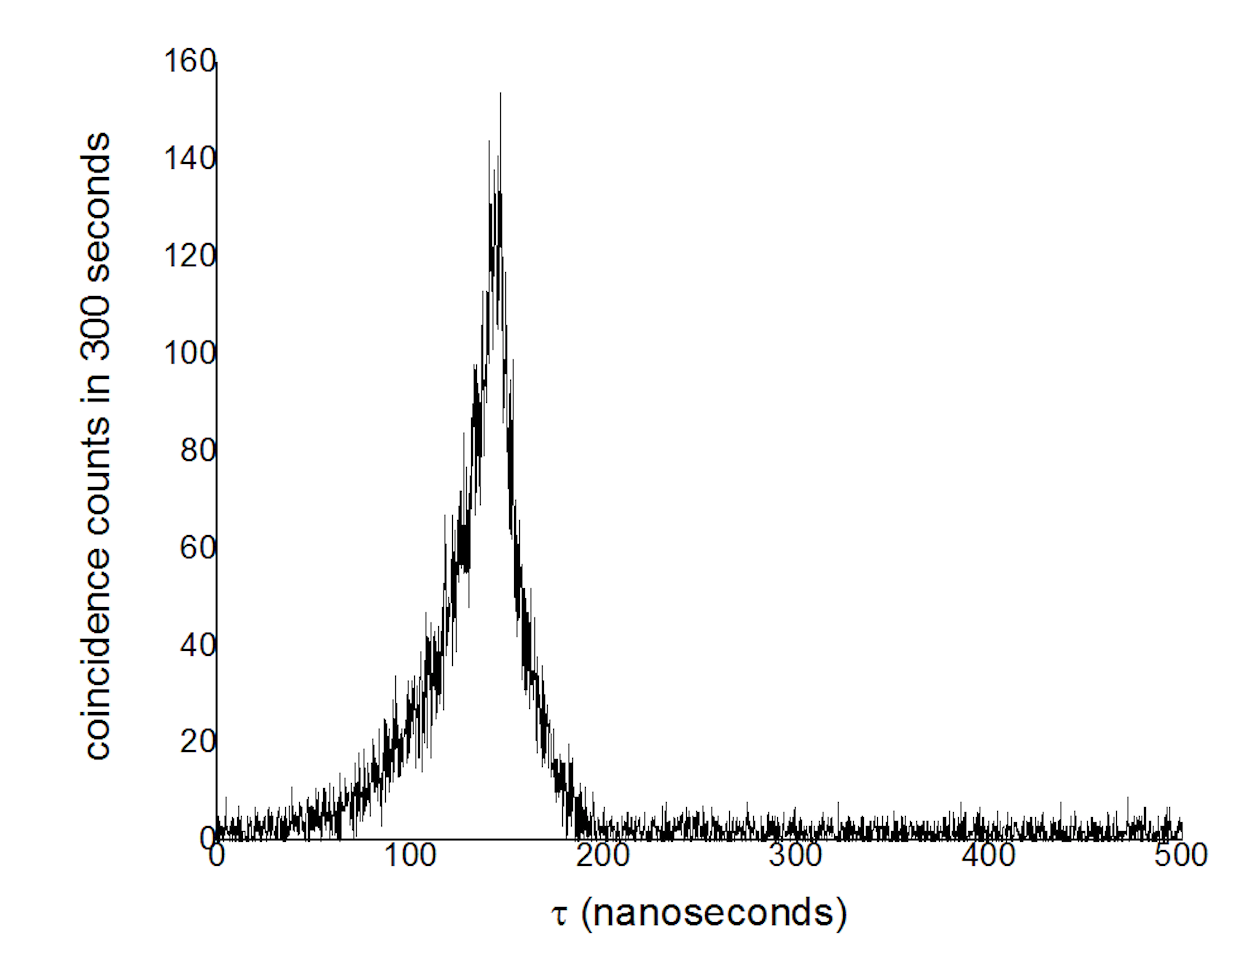
\includegraphics[width=0.3\linewidth]{nocell_no_etalon.png}}
    % ~~~~
    \subcaptionbox
        {只開第一台 EOM
        \label{fig:spread_absorption_g2}}
        {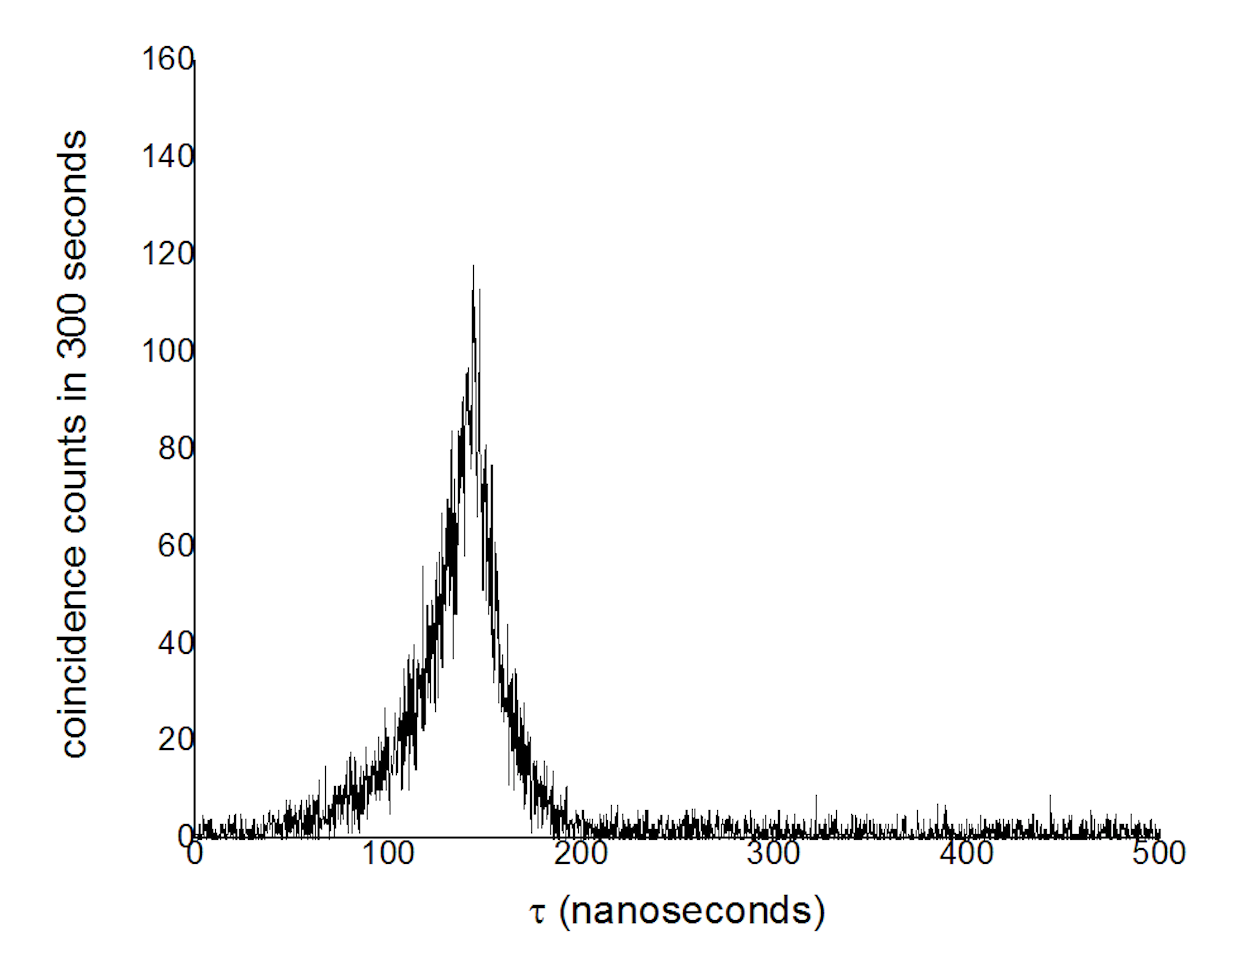
\includegraphics[width=0.4\linewidth]{heatcell_spread_no_etalon.png}}
    ~~~~
    \subcaptionbox
        {同時開啟兩台 EOM
        \label{fig:compress_absorption_g2}}
        {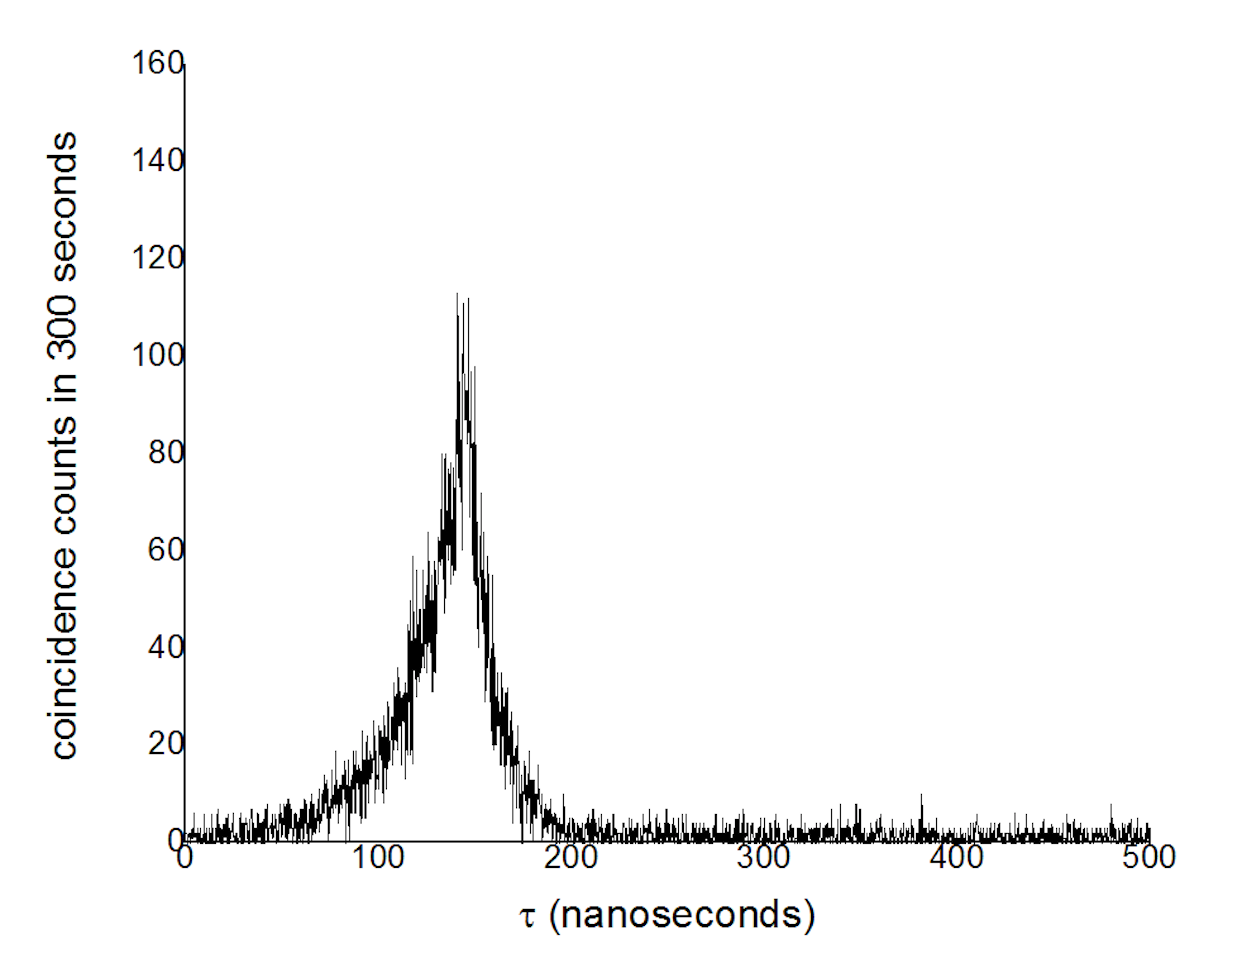
\includegraphics[width=0.4\linewidth]{heatcell_compress_no_etalon.png}}
    \caption{相位調製不影響波形與光強,僅改變頻率的分佈。}
    \label{fig:spread_or_not}
\end{figure}

從前述的結果可知,未經調製的窄頻單光子會幾乎被 $^{87}Rb$ 原子吸收,無法透射氣體管,透射率幾乎為零,但經過 10 Gb/s 隨機訊號的調製後,可讓透射率提升至 76%,如同穿上隱形斗篷般,能大部分的光子不會與原子產生交互作用,直接穿透原子團。

\section{雷射光相位調製對原子吸收之影響}
在上一小節中,我們對單光子進行相位調製,觀察展頻對吸收率之影響,為確定此現象在不同系統下能維持一致性,我們將\cref{fig:single_photon_no_etalon}光路架設的光源改為雷射光,單光子探測器改用光二極體,並將雷射調至與單光子同樣的波長去進行相同的量測,實驗結果如\cref{fig:laser_no_etalon},與單光子的量測結果相近,調製前的光幾乎會全部被原子團吸收,但經過展頻後的雷射光能有約 80\% 的穿透率,也能達到隱形斗篷的效果。

\fig[0.75][fig:laser_no_etalon][!htb]{laser_no_etalon.png}[雷射光相位調製對穿透率之影響,最上面三條線(藍、紅與黃色)為沒放$^{87}RB$ 原子氣體管時之量測,無論是展頻還是壓縮,相位調製皆不會影響光強;中間兩條線(綠色與橘色)為展頻後通過氣體管所測得的訊號,約 80\% 的光能因相位調製而穿透原子團而不被吸收;最下面的藍線為兩台 EOM 關閉時測到的訊號,未經調製的光會幾乎都被原子吸收。][雷射光相位調製對穿透率之影響]

\section{不同展頻頻寬對吸收率之影響}
由\cref{section:simulation_absorption} 的模擬可知,使用越高頻的隨機訊號去展頻可提升光子隱形的效果,為驗證此理論,我們分別使用 2, 4, 6, 8, 10 Gb/s 的隨機訊號去展頻,並透射原子團測量穿透率,實驗結果如\cref{fig:different_gbs_abs},從結果可看出,無論是雷射光或單光子,頻寬越大,吸收率越低,使用越高的頻率去進行調製,的確能增加光子的隱匿性,降低環境或竊聽者的影響。

\fig[0.75][fig:different_gbs_abs][!htb]{main_result.png}[黑色為數值模擬;紅線與藍線分別為雷射光與單光子的實驗測量結果,數據點的值為數次測量的平均,帶狀的寬度為測量的標準差。單光子的實驗結果標準差較大是由於晶體溫控穩定度不夠造成的。][改變展頻頻率對吸收率之影響]

此外,可以看出單光子的透射率皆比雷射光低一些,或許是因為單光子較容易被原子團吸收所致。

\section{單光子頻譜壓縮}

從前兩小節的結果可知,使用展頻技術可以有效的降低環境對光子的影響,但若考量到接收訊息端可能會需要光子原始的相位資訊,或者需要讓光子與 $^{87}Rb$ 原子進行交互作用,我們必須要開啟第二台 EOM 進行反向的調製,盡量使光子還原到原先的狀態,若以\cref{fig:single_photon_no_etalon} 的光路架設,除了第一台 EOM 外,將第二台也開啟,由於相位調製不影響光強與波形,單就 $G^{2}(\tau)$ 的測量無法得知頻譜的變化,因此要將光路架設改為\cref{fig:single_photon_with_etalon},在單光子探測器前加上 Etalon 濾波器,限制只讓頻寬 60 MHz 內的光通過,如此一來,只要能測到訊號就代表部分光子的頻寬有被壓窄至 60 MHz 內,另一方面,這也可以將上一小節及提的雜訊去除。

\fig[0.75][fig:single_photon_with_etalon][!htb]{single_photon_with_etalon_setup.png}[加上濾波器之單光子量測光路圖]

以\cref{fig:single_photon_with_etalon} 的光路架設,只開啟第一台 EOM 時,被展頻的單光子能大部分透射原子團,但由於 Etalon 的過濾,頻寬 10 GHz 的光子幾乎無法抵達探測器,因而測不到明顯的訊號,結果如\cref{fig:spread_single_photon_with_etalon}。若將第二台 EOM 也開啟,將已展頻且被部分吸收的單光子頻譜壓縮,則能再次測到訊號,如\cref{fig:compress_single_photon_with_etalon},與調製前且沒放氣體管時的初始訊號相比,透射率為 42.3\%。

\begin{figure}[!hbt]
    %\captionsetup[subfigure]{labelformat=empty} % 完全隱藏圖號
    \centering
    \subcaptionbox
        {只開啟第一台 EOM,將展頻單光子通過原子團,雖然能大部分透射不被吸收,但由於光子的頻寬 10 GHz,遠小於 Etalon 濾波器的 60 MHz,所以測不到訊號。
        \label{fig:spread_single_photon_with_etalon}}
        {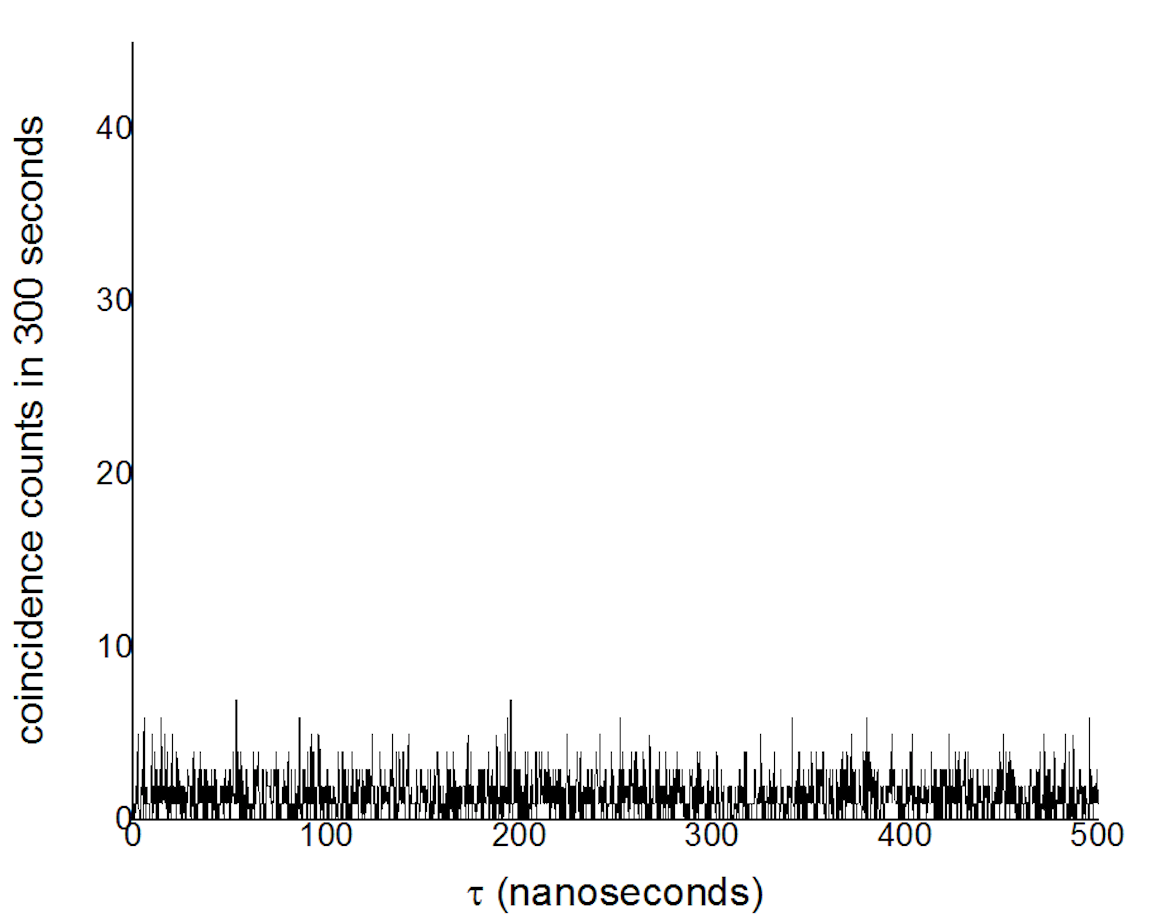
\includegraphics[width=0.4\linewidth]{heat_cell_spread_with_etalon.png}}
    ~~~~
    \subcaptionbox
        {兩台 EOM 同時開啟,將已展頻的單光子頻譜壓縮,使光子再次現形,能透射 Etalon 濾波器,被探測器偵測到。
        \label{fig:compress_single_photon_with_etalon}}
        {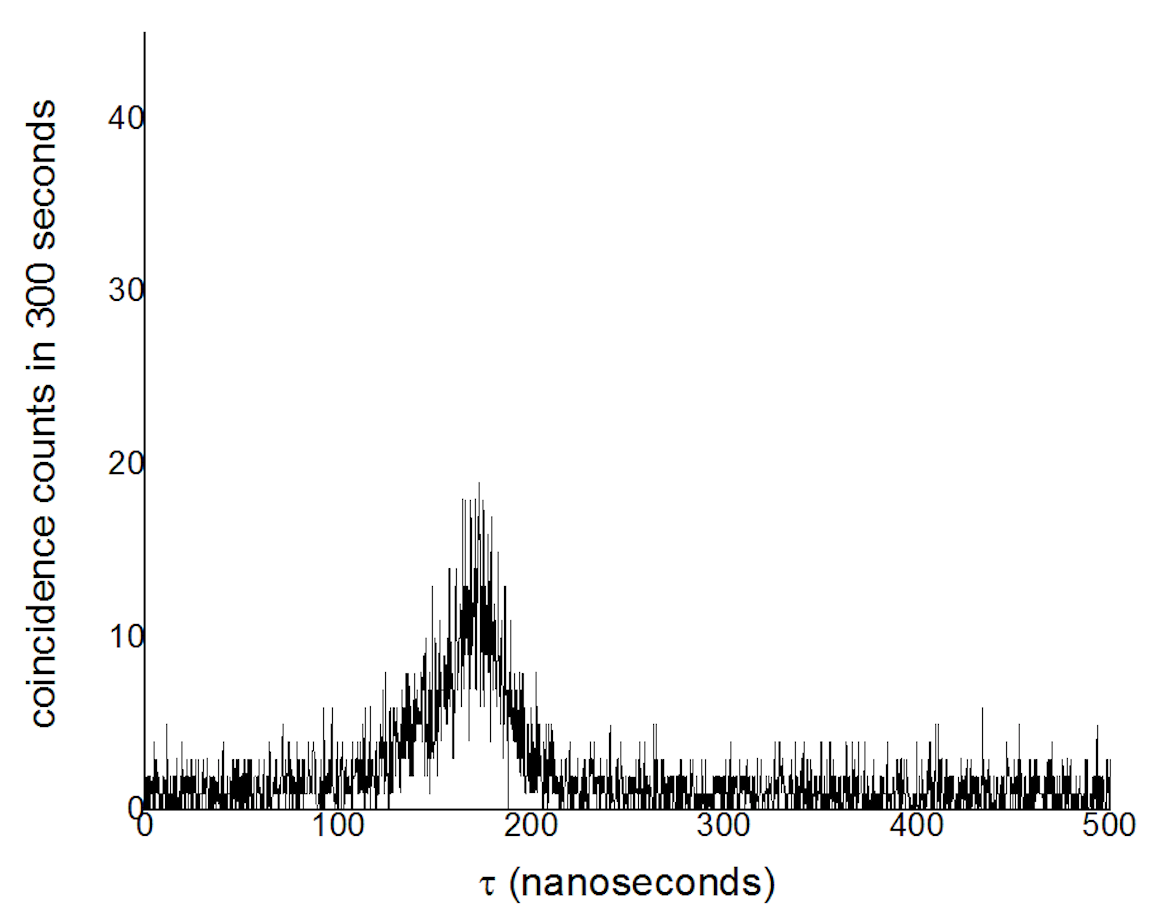
\includegraphics[width=0.4\linewidth]{heat_cell_compress_with_etalon.png}}
    \caption{加上 Etalon 濾波器之單光子 $G^{2}(\tau)$ 量測}
    \label{fig:single_photon_with_etalon}
\end{figure}

為了知道原子吸收對於單光子頻譜的壓縮有何影響,我們以同樣的光路架設,在沒放 $^{87}Rb$ 原子氣體管時同時開啟兩台 EOM,測量結果如\cref{fig:compress_compare_with_etalon}黑線,與調製前的訊號相比,透射率為 77.9\%;放上 $^{87}Rb$ 原子氣體管後的訊號為紅線,透射率為 42.3\%。

\fig[0.75][fig:compress_compare_with_etalon][!htb]{compress_compare_with_etalon.png}[在兩台 EOM 同時開啟時測量 $G^{2}(\tau)$,黑線為沒經過 $^{87}Rb$ 原子氣體管時之量測;紅線為透射 $^{87}Rb$ 原子氣體管之訊號,兩者的比值為 54.3\%。][原子吸收對單光子壓縮比較圖]

\section{雷射光頻譜壓縮}

同樣的,我們以上一小節相同的架設,將光源換成雷射光,單光子探測器改為光二極體,且進行同樣的測量,結果如\cref{fig:no_cell_compress_laser},與單光子的量測結果相近,經展頻後再壓縮的光,約 70\% 能通過 Etalon 濾波器,若在中間放氣體管使部分光被吸收,僅 40\% 的光能通過 Etalon,被重新壓回窄頻雷射

\fig[0.75][fig:no_cell_compress_laser][!htb]{laser_modulation_with_etalon.png}[原子吸收對雷射光壓縮品質比較圖]

\section{誤差分析與模擬修正}

由相位調製的基本原理可知,若輸入兩台 EOM 的隨機訊號符合\cref{eq:prbs_condition} 的條件,則能完美的將光的相位與頻譜還原成最初的狀態,在我們實驗中所使用的窄頻雷射與單光子,頻寬皆遠小於 Etalon 濾波器的頻寬,在沒原子團吸收的狀況下,被展頻再壓縮的光應該要能 100\% 通過 Etalon,這與實驗測量的結果不符,我認為主要的可能原因為隨機訊號的品質不佳所致,兩個訊號從 PRBS 輸出時的波形如\cref{fig:prbs_eye_},兩者形狀不一致,且上下不對稱,若在經過延長線與高頻訊號放大器波形則變為\cref{fig:amp_prbs_eye},兩者變得更不一致,有著不一樣的波形、穩定度、上升時間、下降時間與交叉位置 (crossing),這些因素都會使兩台 EOM 的調製無法互相抵消,讓相位無法還原至最初的狀態。除此之外,也有能是因為兩台 EOM 對高頻訊號的響應不同,也會影響調製的結果。

\begin{figure}[!hbt]
    %\captionsetup[subfigure]{labelformat=empty} % 完全隱藏圖號
    \centering
    \subcaptionbox
        {第一台 EOM
        \label{fig:subfig_fig1}}
        {\includegraphics[width=0.4\linewidth]{data.bmp}}
    ~~~~
    \subcaptionbox
        {第二台 EOM
        \label{fig:subfig_fig2}}
        {\includegraphics[width=0.4\linewidth]{data_bar.bmp}}
    \caption{PRBS 輸出之訊號眼圖(放大前)}
    \label{fig:prbs_eye_}
\end{figure}

\begin{figure}[!hbt]
    %\captionsetup[subfigure]{labelformat=empty} % 完全隱藏圖號
    \centering
    \subcaptionbox
        {第一台 EOM
        \label{fig:subfig_fig1}}
        {\includegraphics[width=0.4\linewidth]{amp_data.bmp}}
    ~~~~
    \subcaptionbox
        {第二台 EOM
        \label{fig:subfig_fig2}}
        {\includegraphics[width=0.4\linewidth]{amp_data_bar.bmp}}
    \caption{PRBS 輸出之訊號眼圖(放大後)}
    \label{fig:amp_prbs_eye}
\end{figure}

為了確認上述的因素所造成的影響,根據\cref{fig:amp_prbs_eye}的測量結果,修正模擬時使用的隨機訊號,修正的參數如\cref{tab:paras},模擬的電訊號如\cref{fig:modify_or_not}。

\begin{figure}[!hbt]
    %\captionsetup[subfigure]{labelformat=empty} % 完全隱藏圖號
    \centering
    \subcaptionbox
        {修正前
        \label{fig:subfig_fig1}}
        {
\includegraphics[width=0.4\linewidth]{temp.png}}
    ~~~~
    \subcaptionbox
        {修正後
        \label{fig:subfig_fig2}}
        {
\includegraphics[width=0.4\linewidth]{temp.png}}
    \caption{理論模擬使用的隨機訊號}
    \label{fig:modify_or_not}
\end{figure}

使用修正後的隨機訊號進行展頻、吸收與壓縮的模擬,可讓計算的結果更貼近實驗的測量,以下將整理理論與實驗的結果整理成\cref{tab:spread_abs} 與\cref{tab:compress_abs},從表中可觀察到,經過修正後的理論模擬更接近實驗的結果,由此可知,想要有效地使用展頻技術,電訊號的品質起了關鍵的作用,需要有更好的訊號產生器與線材才可以將調製的訊號還原成原始的模樣。

\begin{table}[h]
    \centering
    \caption{數值模擬參數修正}
    \begin{tabular}{| c | c | c | c |}
\hline
         & jitter & amplitidu & rising \& falling
    \\ \hline
    \ce{EOM 1} & 14 ps & $\pm$7.7\% & 38 ps\\ \hline
    \ce{EOM 2} & 16 ps & $\pm$16.7\% & 144 ps\\ \hline
    \end{tabular}
    \label{tab:paras}
\end{table}

\begin{table}[h]
    \centering
    \caption{展頻後的光經過 $^{87}Rb$ 原子氣體管之透射率(無 Etalon 濾波器)}
    \begin{tabular}{| c | c | c | c | c |}
\hline
\multirow{2}{*}{無 Etalon}& \multicolumn{2}{c|}{ 理論 } & \multicolumn{2}{c|}{ 實驗 }
\\ \cline{2-5}
         & 修正前 & 修正後 & 雷射光 & 單光子
    \\ \hline
    穿透率 & 79.1\% & 73.8\% & 77.38\% & 68.48\%\\ \hline
    \end{tabular}
    \label{tab:spread_abs}
\end{table}

\begin{table}[h]
    \centering
    \caption{展頻後壓縮的光經過 Etalon 濾波器之透射率}
    \begin{tabular}{| c | c | c | c | c |}
\hline
    \multirow{2}{*}{有 Etalon}& \multicolumn{2}{c|}{ 理論 } & \multicolumn{2}{c|}{ 實驗 }
    \\ \cline{2-5}
        & 修正前 & 修正後 & 雷射光 & 單光子
    \\ \hline
    無通過氣體管 & 100.0\% & 88.9\% & 77.9\% & 70.9\%\\ \hline
    有通過氣體管 & 67.6\% & 45.6\% & 42.3\% & 41.0\%\\ \hline
    \end{tabular}
    \label{tab:compress_abs}
\end{table}

\todo[inline]{補上模擬圖}
\end{document}